        %%******************************************%%
        %%                                          %%
        %%        Modello di tesi di laurea         %%
        %%            di Andrea Giraldin            %%
        %%                                          %%
        %%             2 novembre 2012              %%
        %%                                          %%
        %%******************************************%%

\begin{document}
    \frontmatter
    \begin{titlepage}
    \begin{center}
        \begin{LARGE}
            \textbf{\myUni}\\
        \end{LARGE}

        \vspace{10pt}

        \begin{Large}
            \textsc{\myDepartment}\\
        \end{Large}

        \vspace{10pt}

        \begin{large}
            \textsc{\myFaculty}\\
        \end{large}

        \vspace{30pt}
        \begin{figure}[htbp]
            \centering
            \includegraphics[height=6cm]{unipd-logo}
        \end{figure}
        \vspace{30pt}

        \begin{LARGE}
            \textbf{\myTitle}\\
        \end{LARGE}

        \vspace{10pt}

        \begin{large}
            \textsl{\myDegree}\\
        \end{large}

        \vspace{40pt}

        \begin{large}
            \begin{flushleft}
                \textit{Relatore}\\
                \vspace{5pt}
                \profTitle\ \myProf
            \end{flushleft}

            % You can tweak the spacing to have professor and student names on the same line
            % useful if the page is broken by a long thesis title and you need more space
            % \vspace{-52pt}

            \begin{flushright}
                \textit{Laureando}\\
                \vspace{5pt}
                \myName \\
                \vspace{5pt}
                \textit{Matricola} \myID
            \end{flushright}
        \end{large}

        \vspace{40pt}

        \line(1, 0){338} \\
        \begin{normalsize}
            \textsc{Anno Accademico \myAA}
        \end{normalsize}
    \end{center}
\end{titlepage}

    \input{preface/copyright}
    \cleardoublepage
\phantomsection
\thispagestyle{empty}
\pdfbookmark{Dedica}{Dedica}

\vspace*{3cm}

\begin{center}
    Lorem ipsum dolor sit amet, consectetuer adipiscing elit. \\ \medskip
    --- Oscar Wilde
\end{center}

\medskip

%\begin{center}
%    Dedicato a ...
%\end{center}

    \cleardoublepage
\phantomsection
\pdfbookmark{Sommario}{Sommario}
\begingroup
\let\clearpage\relax
\let\cleardoublepage\relax
\let\cleardoublepage\relax

\chapter*{Sommario}

Il presente documento descrive il lavoro svolto durante il periodo di stage, della durata di trecentoventi ore, dal laureando Marco Cola presso l'azienda Kirey S.r.l.
Gli obbiettivi da raggiungere erano molteplici.\\
In primo luogo era richiesto lo sviluppo di ...
In secondo luogo era richiesta l'implementazione di un ...
Tale framework permette di registrare gli eventi di un controllore programmabile, quali segnali applicati
Terzo ed ultimo obbiettivo era l'integrazione ...

%\vfill

%\selectlanguage{english}
%\pdfbookmark{Abstract}{Abstract}
%\chapter*{Abstract}

%\selectlanguage{italian}

\endgroup

\vfill

    \cleardoublepage
\phantomsection
\pdfbookmark{Ringraziamenti}{ringraziamenti}

\begin{flushright}{
    \slshape
    ``Quando incontri un uomo con la spada, estrai la tua spada: \\
    non recitare poesie a chi non è poeta''} \\
    \medskip
    --- proverbio Ch'an
\end{flushright}


\bigskip

\begingroup
\let\clearpage\relax
\let\cleardoublepage\relax
\let\cleardoublepage\relax

\chapter*{Ringraziamenti}

\noindent \textit{Innanzitutto, vorrei esprimere la mia gratitudine al Prof. \myProf, relatore della mia tesi, per l'aiuto e il sostegno fornitomi durante la stesura del lavoro.}\\

\noindent \textit{Desidero ringraziare con affetto i miei genitori per il sostegno, il grande aiuto e per essermi stati vicini in ogni momento durante gli anni di studio.}\\

%\noindent \textit{Ho desiderio di ringraziare poi i miei amici per tutti i bellissimi anni passati insieme e le mille avventure vissute.}\\
\bigskip

\noindent\textit{\myLocation, \myTime}
\hfill \myName

\endgroup

    \input{preface/table-of-contents}
    \cleardoublepage

    \mainmatter
    \chapter{Introduzione}
\label{cap:introduzione}

Introduzione al contesto applicativo.\\

\noindent Esempio di utilizzo di un termine nel glossario \\
\gls{api}. \\

\noindent Esempio di citazione in linea \\
\cite{site:agile-manifesto}. \\

\noindent Esempio di citazione nel pie' di pagina \\
citazione\footcite{womak:lean-thinking} \\

\section{L'azienda}
Kirey Group è uno dei \emph{system integrator} europei più dinamici e in crescita, specializzato nell'accompagnare le imprese nei percorsi di trasformazione digitale
 e di adozione di modelli \emph{data-driven}. Con sede principale in Italia e una presenza consolidata in diversi Paesi europei ed extraeuropei, 
 il Gruppo conta oltre 1000 professionisti e opera in dieci Paesi.

\begin{figure}[!h] 
    \centering 
    
\includegraphics[width=0.9\columnwidth]{Kirey_logo.jpg} 
    \caption{Figura 1 - Logo di Kirey S.r.l.}
\end{figure}

La missione di Kirey è rendere l'innovazione accessibile, trasformando il potenziale tecnologico in valore economico e in nuovi modelli di business. 
L'azienda si distingue per un approccio che unisce affidabilità tecnica, innovazione guidata dai dati, competenza centrata sull'uomo e sinergia cross-funzionale, 
elementi che costituiscono i valori fondanti del marchio.

Il manifesto del gruppo sintetizza questa filosofia nel concetto “\emph{Data Made Human}”, ovvero la volontà di tradurre la complessità dei dati in soluzioni comprensibili, 
intuitive e ad alto impatto, mettendo sempre la persona al centro della tecnologia.

La storia del gruppo affonda le radici negli anni Settanta e, attraverso fusioni, acquisizioni e nuove fondazioni, ha portato alla nascita di Kirey Group nel 2016. 
Negli anni successivi l'azienda ha accelerato la propria espansione internazionale integrando nuove realtà, consolidando così competenze e capacità operative in diversi settori e mercati

Il portafoglio di servizi è ampio e integrato, con \emph{Data \& AI} come filo conduttore e aree principali che comprendono:

\begin{itemize}
    \item \emph{Cloud \& Infrastructure}, con soluzioni ibride e \emph{on-premise}, sicurezza in ambienti \emph{cloud}, migrazione e monitoraggio;
    \item \emph{Software Development}, che spazia dallo sviluppo agile e mobile alla \emph{system integration}, con particolare attenzione alla qualità e all'automazione dei \emph{test};
    \item \emph{Cybersecurity}, con servizi di consulenza, \emph{audit}, architetture sicure, \emph{managed services} e sistemi antifrode;
    \item \emph{Data \& AI}, che include \emph{data integration}, \emph{data governance}, \emph{analytics}, \emph{machine learning}, \emph{synthetic data}, \emph{forecasting} e soluzioni \gls{esg}.
\end{itemize}

Kirey Group pone grande attenzione alla sostenibilità, alla trasparenza e all'integrità, adottando pratiche responsabili nei confronti di clienti, partner, dipendenti e \emph{stakeholder}. 
L'azienda è inoltre attivamente impegnata in progetti sociali, promuove la diversità e l'inclusione, e investe nello sviluppo delle competenze tecnologiche e professionali delle proprie persone.

Oggi il gruppo conta oltre 1370 casi di business realizzati, 10 \emph{Innovation Center} attivi, un fatturato di circa 126 milioni di euro e più di 1000 collaboratori distribuiti in 10 paesi.


\section{L'idea}

Introduzione all'idea dello stage.

\section{Organizzazione del testo}

\begin{description}
    \item[{\hyperref[cap:processi-metodologie]{Il secondo capitolo}}] descrive ...
    
    \item[{\hyperref[cap:descrizione-stage]{Il terzo capitolo}}] approfondisce ...
    
    \item[{\hyperref[cap:analisi-requisiti]{Il quarto capitolo}}] approfondisce ...
    
    \item[{\hyperref[cap:progettazione-codifica]{Il quinto capitolo}}] approfondisce ...
    
    \item[{\hyperref[cap:verifica-validazione]{Il sesto capitolo}}] approfondisce ...
    
    \item[{\hyperref[cap:conclusioni]{Nel settimo capitolo}}] descrive ...
\end{description}

Riguardo la stesura del testo, relativamente al documento sono state adottate le seguenti convenzioni tipografiche:
\begin{itemize}
	\item gli acronimi, le abbreviazioni e i termini ambigui o di uso non comune menzionati vengono definiti nel glossario, situato alla fine del presente documento;
	\item per la prima occorrenza dei termini riportati nel glossario viene utilizzata la seguente nomenclatura: \emph{parola}\glsfirstoccur;
	\item i termini in lingua straniera o facenti parti del gergo tecnico sono evidenziati con il carattere \emph{corsivo}.
\end{itemize}

    %\input{chapters/processi}
    \chapter{Descrizione dello stage}
\label{cap:descrizione-stage}

\intro{Il capitolo approfondisce il progetto di stage, descrivendo gli obiettivi e le attività svolte, la metodologia di lavoro adottata e un'analisi preventiva dei principali rischi e relative strategie di mitigazione.}\\

\section{Introduzione al progetto}
Lo stage è stato svolto presso l'azienda Kirey Group S.r.l., realtà consolidata nell'ambito della fornitura di prodotti e servizi informatici, con clienti internazionali e una forte specializzazione nei settori \emph{Banking}, \emph{Insurance}, \emph{Oil\&Gas} e Pubblica Amministrazione. \\ 
L'attività si è inserita nel contesto del team \gls{apm}\glsfirstoccur e ha avuto come obiettivo principale la realizzazione e il collaudo di una piattaforma per il monitoraggio delle performance di una \emph{web application}. \\
Il progetto è stato sviluppato interamente in ambiente \emph{Linux} mediante \emph{Windows Subsystem for Linux}, utilizzando la \emph{suite} \emph{Elastic Stack} e i suoi principali componenti: \emph{Elasticsearch} per la gestione dei dati, \emph{Kibana} per la visualizzazione, \emph{Logstash} per l'ingestione e la trasformazione dei log, \emph{Beats} e \emph{Fleet Server} per la raccolta distribuita delle metriche e \emph{APM Server/Agent} per il tracciamento delle \emph{performance} applicative. \\ 
Sono stati realizzati sviluppi in \emph{Python} e \emph{Java} per l'estensione delle funzionalità e l'integrazione di algoritmi di \gls{ai}\glsfirstoccur e \emph{Machine Learning}, con l'obiettivo di rilevare automaticamente anomalie e problematiche di prestazione. \\   
La finalità complessiva è quella di fornire un sistema scalabile, proattivo e ben documentato, capace di garantire prestazioni ottimali e un monitoraggio continuo della \emph{web application}.  


\section{Pianificazione}
Tutte le attività sono state condotte in affiancamento ad un tutor aziendale che ha curato sia la parte di formazione che di indirizzamento delle attività.
A tal fine sono stati svolti dei momenti di confronto settimanali per la valutazione dello stato di avanzamento delle attività e momenti quotidiani di confronto sulle problematiche riscontrate. \\
Le attività proposte sono state collocate all'interno di un progetto più ampio portato avanti in Kirey da un team di persone eterogeneo. \\
Al termine dello stage sono stati presentati i risultati ottenuti a tutto il team.
L'infrastruttura tecnologica e le piattaforme su cui girerà l'applicazione sono state messe a disposizione da Kirey.


\section{Analisi preventiva dei rischi}

Durante la fase di analisi iniziale sono stati individuati alcuni possibili rischi a cui si potrà andare incontro.
Si è quindi proceduto a elaborare delle possibili soluzioni per far fronte a tali rischi.\\

\begin{risk}{Inesperienza nella suite Elastic}
    \vspace{0.5em}
    \riskdescription{La limitata esperienza iniziale nell'utilizzo della \emph{Elastic Stack} (\emph{Elasticsearch}, \emph{Kibana}, \emph{Logstash}, \emph{APM}) potrebbe comportare difficoltà nella configurazione e nell'integrazione delle componenti, rallentando lo sviluppo del progetto}
    \vspace{0.5em}
    \riskimpact{Alto}
    \vspace{0.5em}
    \riskprobability{Alta}
    \vspace{0.5em}
    \risksolution{Organizzazione di momenti di confronto con il tutor aziendale e studio personale della documentazione, al fine di acquisire le competenze necessarie}
    \label{risk:elastic-inexperience}
\end{risk}

\vspace{1em}

\begin{risk}{Integrazione tra componenti Elastic}
    \vspace{0.5em}
    \riskdescription{La comunicazione tra i diversi moduli della \emph{suite} \emph{Elastic} (\emph{Elasticsearch}, \emph{Kibana}, \emph{Logstash}, \emph{APM}) potrebbe presentare problemi di configurazione, causando ritardi o malfunzionamenti nell'acquisizione dei dati}
    \vspace{0.5em}
    \riskimpact{Medio}
    \vspace{0.5em}
    \riskprobability{Media}
    \vspace{0.5em}
    \risksolution{Esecuzione di test di connettività e validazione progressiva delle \emph{pipeline}, con il supporto del \emph{tutor} aziendale per la risoluzione dei problemi}
    \label{risk:elastic-integration}
\end{risk}

\vspace{1em}

\begin{risk}{Qualità e coerenza dei dati raccolti}
    \vspace{0.5em}
    \riskdescription{I dati acquisiti dagli agenti potrebbero risultare incompleti, duplicati o non coerenti, compromettendo le analisi e le \emph{dashboard}}
    \vspace{0.5em}
    \riskimpact{Alto}
    \vspace{0.5em}
    \riskprobability{Media}
    \vspace{0.5em}
    \risksolution{Definizione di regole di filtraggio e validazione all'interno delle \emph{pipeline} \emph{Logstash} ed esecuzione di test di integrità sugli indici \emph{Elasticsearch}}
    \label{risk:data-quality}
\end{risk}

\vspace{1em}

\begin{risk}{Scalabilità e carico del sistema}
    \vspace{0.5em}
    \riskdescription{L'aumento del volume dei dati e delle richieste potrebbe impattare sulle prestazioni della piattaforma, riducendo l'efficienza del monitoraggio}
    \vspace{0.5em}
    \riskimpact{Medio}
    \vspace{0.5em}
    \riskprobability{Media}
    \vspace{0.5em}
    \risksolution{Implementazione di strategie di \emph{scaling} orizzontale e utilizzo di metriche di \emph{Kibana} per monitorare l'impatto del carico in tempo reale}
    \label{risk:scalability}
\end{risk}

\vspace{1em}

\begin{risk}{Implementazione di algoritmi di Machine Learning}
    \vspace{0.5em}
    \riskdescription{L'integrazione di modelli di \emph{Machine Learning} per il rilevamento delle anomalie potrebbe richiedere competenze specifiche e tempi di sviluppo più lunghi del previsto}
    \vspace{0.5em}
    \riskimpact{Alto}
    \vspace{0.5em}
    \riskprobability{Media}
    \vspace{0.5em}
    \risksolution{Formazione preliminare su tecniche di \emph{Machine Learning} e utilizzo di librerie e \emph{framework} consolidati per accelerare lo sviluppo}
    \label{risk:ml-implementation}
\end{risk}

\vspace{1em}

\begin{risk}{Problemi di configurazione delle pipeline Logstash}
    \vspace{0.5em}
    \riskdescription{Errori di configurazione nelle \emph{pipeline} di \emph{Logstash} potrebbero causare la perdita, la duplicazione o la trasformazione errata dei dati raccolti, compromettendo l'affidabilità delle analisi}
    \vspace{0.5em}
    \riskimpact{Alto}
    \vspace{0.5em}
    \riskprobability{Media}
    \vspace{0.5em}
    \risksolution{Adozione di un approccio con \emph{test} di validazione a ogni modifica delle \emph{pipeline} e utilizzo di ambienti di prova per verificare la correttezza del flusso dei dati prima della messa in produzione}
    \label{risk:logstash-pipeline}
\end{risk}

\vspace{1em}

\begin{risk}{Accesso limitato a funzionalità premium di Elastic}
    \vspace{0.5em}
    \riskdescription{Durante le prime settimane di lavoro in locale, la mancata possibilità di operare su \emph{Elastic Cloud} e di accedere a funzionalità premium come il \emph{Machine Learning} potrebbe limitare l'analisi dei dati e rallentare la validazione di alcune funzionalità previste dal progetto}
    \vspace{0.5em}
    \riskimpact{Medio}
    \vspace{0.5em}
    \riskprobability{Bassa}
    \vspace{0.5em}
    \risksolution{Esecuzione preventiva delle attività in locale con dati di test, studio della documentazione sulle funzionalità premium e pianificazione di un passaggio successivo a \emph{Elastic Cloud} non appena disponibile, con supporto del tutor aziendale}
    \label{risk:elastic-cloud-limitations}
\end{risk}


\section{Requisiti e obiettivi}
Gli obiettivi del progetto sono stati classificati in base alla loro priorità secondo le seguenti notazioni:

\begin{itemize}
    \item \textbf{Ob} (Requisiti Obbligatori) - requisiti essenziali e imprescindibili per il successo del progetto, vincolanti in quanto obiettivo primario richiesto dal committente;
    \item \textbf{D} (Requisiti Desiderabili) - requisiti importanti ma non critici, la cui assenza non compromette il progetto, non vincolanti o strettamente necessari, ma dal riconoscibile valore aggiunto;
    \item \textbf{Op} (Requisiti Opzionali) - requisiti desiderabili ma non essenziali, rappresentanti valore aggiunto non strettamente competitivo.
\end{itemize}

\vspace{1em}

Durante il periodo di stage si prevede il raggiungimento dei seguenti obiettivi:

\begin{itemize}
    \item \textbf{Preparazione dell'ambiente per l'implementazione della soluzione:}  
        \begin{itemize}
            \item \textbf{Ob1.1:} Individuazione delle componenti ed eventuali librerie da utilizzare;
            \item \textbf{Ob1.2:} Installazione e configurazione delle componenti;
            \item \textbf{Ob1.3:} Verifica del corretto funzionamento dell'ambiente e test di connettività tra componenti.
        \end{itemize}
    \item \textbf{Implementazione estrazione dati dalla web application:}  
        \begin{itemize}
            \item \textbf{Ob2.1:} Configurazione \emph{agent} (\emph{Beats/APM}) per la raccolta dati della navigazione;
            \item \textbf{Ob2.2:} Implementazione \emph{pipeline} di \emph{log} tramite \emph{Logstash} per filtraggio e inoltro dati in \emph{Elasticsearch};
            \item \textbf{Ob2.3:} Verifica della corretta acquisizione dei dati e loro indicizzazione in \emph{Elasticsearch}.
        \end{itemize}
    \item \textbf{Implementazione elaborazione dati e rappresentazione grafica dei dati:}  
        \begin{itemize}
            \item \textbf{Ob3.1:} Sviluppo \emph{script} \emph{Python/Java} per il monitoraggio sintetico (\emph{Selenium}) e generazione di traffico \emph{log};
            \item \textbf{Ob3.2:} Analisi e aggregazione dati in \emph{Elasticsearch}, con \emph{query} e visualizzazioni preliminari;
            \item \textbf{Ob3.3:} Creazione dashboard avanzate su \emph{Kibana} con metriche di \emph{performance}, accesso e flussi utente;
            \item \textbf{Op3.4:} Configurazione regole di \emph{alerting} e notifiche per anomalie rilevate in tempo reale.
        \end{itemize}
    \item \textbf{Documentazione dettagliata:}  
        \begin{itemize}
            \item \textbf{Ob4.1:} Descrizione delle tecnologie e prodotti utilizzati;
            \item \textbf{Ob4.2:} Descrizione dei flussi logici del progetto e delle funzionalità dell'applicazione;
            \item \textbf{D4.3:} Pro/contro di ogni componente e criticità nell'applicazione.
        \end{itemize}
\end{itemize} 
Nel capitolo successivo verrà approfondita l'analisi dei requisiti identificati in questa sezione, al fine di definirne in modo più strutturato la natura e le caratteristiche.
    \chapter{Analisi dei requisiti}
\label{cap:analisi-requisiti}

\intro{Il capitolo è dedicato all'analisi dei requisiti della piattaforma, con l'obiettivo di fornire una visione completa e dettagliata delle funzionalità e delle caratteristiche attese dal sistema. Verranno illustrate le esigenze degli utenti e del contesto operativo, evidenziando le specifiche tecniche e le funzionalità che hanno guidato le scelte progettuali.}\\

%\section{Casi d'uso}

%Per lo studio dei casi di utilizzo del prodotto sono stati creati dei diagrammi.
%I diagrammi dei casi d'uso (in inglese \emph{Use Case Diagram}) sono diagrammi di tipo \gls{uml}\glsfirstoccur dedicati alla descrizione delle funzioni o servizi offerti da un sistema, così come sono percepiti e utilizzati dagli attori che interagiscono col sistema stesso. \\
%Nel contesto del progetto, volto alla creazione di una piattaforma di monitoraggio per applicazioni \emph{web} con strumenti di \gls{apmg} e componenti di intelligenza artificiale per l’analisi automatica dei dati, le interazioni da parte dell’utente sono ridotte allo stretto necessario. Questo approccio minimizza l’intervento manuale, garantendo che le funzionalità principali siano accessibili in maniera intuitiva e diretta. Di conseguenza, i diagrammi dei casi d’uso risultano semplici e in numero limitato, focalizzati sulle operazioni essenziali per la raccolta, l’analisi e la visualizzazione dei dati di monitoraggio.

%\begin{figure}[!h] 
    %\centering 
    %\includegraphics[width=0.9\columnwidth]{usecase/scenario-principale} 
    %\caption{Use Case - UC0: Scenario principale}
%\end{figure}

%\begin{usecase}{0}{Scenario principale}
%\usecaseactors{Sviluppatore applicativi}
%\usecasepre{Lo sviluppatore è entrato nel plug-in di simulazione all'interno dell'IDE}
%\usecasedesc{La finestra di simulazione mette a disposizione i comandi per configurare, registrare o eseguire un test}
%\usecasepost{Il sistema è pronto per permettere una nuova interazione}
%\label{uc:scenario-principale}
%\end{usecase}

\section{Requisiti del sistema}

A seguito di un'attenta attività di analisi del progetto e degli obiettivi tecnici e funzionali prefissati, sono state redatte le tabelle di tracciamento che riassumono in modo strutturato i requisiti individuati. \\
Durante questa fase sono state identificate differenti tipologie di requisiti, distinte sia in base alla loro categoria (funzionale, non funzionale, qualitativo o di vincolo), sia in base alla loro priorità di implementazione (obbligatorio, desiderabile o opzionale).
Per garantire una tracciabilità chiara e univoca, a ciascun requisito è stato assegnato un codice identificativo composto da lettere che ne descrivono la tipologia e l'importanza, secondo la seguente convenzione:
\begin{description}
	\item [R =] Requisito
	\item [F =] Funzionale
    \item [N =] Non funzionale
    \item [Q =] Qualitativo
    \item [V =] Vincolo
    \item [O =] Obbligatorio
    \item [D =] Desiderabile
    \item [Z =] Opzionale
\end{description}

\newpage

Ogni requisito analizzato sarà identificato univocamente dalla seguente notazione:
\begin{center}
    \textbf{R[Priorità][Categoria]-[Numero]}
\end{center}
Dove:

\begin{itemize}
    \item \textbf{Priorità} indica la priorità di implementazione, che può essere O = Obbligatorio, D = Desiderabile, Z = Opzionale;
    \item \textbf{Categoria} la categoria di appartenenza, che può essere F = Funzionale, N = Non funzionale, Q = Qualitativo, V = Vincolo;
    \item \textbf{Numero} un numero progressivo che identifica in modo univoco il requisito all'interno della sua categoria.
\end{itemize}
Nelle tabelle \ref{tab:requisiti-funzionali}, \ref{tab:requisiti-non-funzionali}, \ref{tab:requisiti-qualitativi} e \ref{tab:requisiti-vincolo} sono riportati in modo sintetico tutti i requisiti emersi dall'analisi, classificati in base alla loro priorità e accompagnati da una breve descrizione della relativa funzionalità o vincolo tecnico. \\


\newpage
\subsection{Requisiti funzionali}
I requisiti funzionali descrivono cosa deve fare il sistema.
Sono le funzionalità concrete che la soluzione deve offrire per raggiungere gli obiettivi del progetto.

\begin{table}[h]
\caption{Tabella del tracciamento dei requisiti funzionali}
\label{tab:requisiti-funzionali}
\begin{tabularx}{\textwidth}{lXl}
\hline
\rowcolor[gray]{0.8}
\textbf{Codice} & \textbf{Descrizione} & \textbf{Classificazione}\\
\hline
ROF-1     & Il sistema deve permettere la raccolta automatica di metriche e \emph{log} relativi alla \emph{web application} tramite agenti \emph{OpenTelemetry} o \emph{Elastic APM}. & Obbligatorio \\
\hline

\hline
ROF-2     & Il sistema deve inviare i dati raccolti agli \emph{endpoint} \emph{Elasticsearch} per l'analisi e l'indicizzazione. & Obbligatorio \\
\hline

\hline
ROF-3     & Il sistema deve consentire la creazione di \emph{pipeline} di \emph{log} tramite \emph{Logstash} per filtraggio, trasformazione e inoltro dei dati in \emph{Elasticsearch}. & Obbligatorio \\
\hline

\hline
ROF-4     & Il sistema deve prevedere la configurazione di \emph{Elastic Agents} (\emph{Beats}/\emph{\gls{apm}}) per la raccolta dati della navigazione. & Obbligatorio \\
\hline

\hline
ROF-5     & Il sistema deve generare \emph{dashboard} avanzate e visualizzazioni in \emph{Kibana}, con metriche di \emph{performance}, accesso e flussi utente. & Obbligatorio \\
\hline

\hline
ROF-6     & Il sistema deve permettere la verifica della corretta acquisizione dei dati e la loro indicizzazione in \emph{Elasticsearch}. & Obbligatorio \\
\hline

\hline
ROF-7     & Il sistema deve prevedere lo sviluppo e l'esecuzione di \emph{script} automatizzati in \emph{Python} o \emph{Java} per la simulazione del traffico utente (\emph{Synthetic Monitoring}). & Obbligatorio \\
\hline

\hline
ROF-8     & Deve essere possibile filtrare e ricercare i \emph{log} per \emph{host}, servizio, livello di severità o periodo temporale. & Obbligatorio \\
\hline

\hline
RDF-9     & Il sistema dovrebbe prevedere la configurazione di regole di \emph{alerting} e notifiche in tempo reale per anomalie rilevate. & Desiderabile \\
\hline

\hline
RDF-10     & Il sistema dovrebbe integrare algoritmi di \emph{Machine Learning} per l'individuazione automatica di anomalie. & Desiderabile \\
\hline

\hline
RDF-11     & Il sistema dovrebbe consentire l'esportazione delle \emph{dashboard} o dei risultati delle \emph{query} in formato \gls{pdf}\glsfirstoccur o \gls{csv}\glsfirstoccur. & Desiderabile \\
\hline

\hline
RZF-12     & Il sistema può prevedere un modulo aggiuntivo per la generazione automatica di report periodici delle metriche raccolte. & Opzionale \\
\hline

\hline
RZF-13     & Il sistema può consentire l'importazione automatica delle configurazioni \gls{apm} da ambienti di \emph{test} o \emph{staging}. & Opzionale \\
\hline

\end{tabularx}
\end{table}%

\newpage
\subsection{Requisiti non funzionali}
I requisiti non funzionali definiscono come il sistema deve comportarsi, cioè le sue proprietà di qualità interna.
Non aggiungono nuove funzioni, ma impongono vincoli di prestazioni, sicurezza, disponibilità, scalabilità, affidabilità e manutenibilità.

\begin{table}[h]
\caption{Tabella del tracciamento dei requisiti non funzionali}
\label{tab:requisiti-non-funzionali}
\begin{tabularx}{\textwidth}{lXl}
\hline
\rowcolor[gray]{0.8}
\textbf{Codice} & \textbf{Descrizione} & \textbf{Classificazione}\\
\hline
RON-1    & Il sistema deve essere scalabile e consentire l'aggiunta di nuove fonti di dati o agenti senza compromettere la stabilità. & - Obbligatorio \\
\hline

\hline
RON-2    & Il sistema deve garantire l'affidabilità nella trasmissione e nella conservazione dei dati raccolti. & - Obbligatorio \\
\hline

\hline
RON-3    & La piattaforma deve assicurare un tempo di latenza accettabile nella visualizzazione dei dati (< 5 secondi per l'aggiornamento delle \emph{dashboard}). & - Obbligatorio \\
\hline

\hline
RDN-4    & Il sistema dovrebbe garantire la possibilità di eseguire \emph{test} di carico e stress per valutare la stabilità dell'ambiente. & - Desiderabile \\
\hline

\hline
RDN-5    & Il sistema dovrebbe supportare l'autenticazione per la gestione degli accessi a \emph{Kibana}. & - Desiderabile \\
\hline


\end{tabularx}
\end{table}%


\newpage
\subsection{Requisiti qualitativi}
I requisiti qualitativi specificano le proprietà qualitative che influenzano l'esperienza d'uso e la manutenibilità.
Si concentrano su aspetti percepibili, come semplicità, chiarezza, flessibilità o estendibilità.

\begin{table}[h]
\caption{Tabella del tracciamento dei requisiti qualitativi}
\label{tab:requisiti-qualitativi}
\begin{tabularx}{\textwidth}{lXl}
\hline
\rowcolor[gray]{0.8}
\textbf{Codice} & \textbf{Descrizione} & \textbf{Use Case}\\
\hline
ROQ-1    & L'interfaccia di \emph{Kibana} deve offrire una rappresentazione chiara e intuitiva delle metriche principali. & - Obbligatorio \\
\hline

\hline
ROQ-2    & I dati devono essere visualizzabili in forma aggregata e filtrabile in base a intervalli temporali e categorie di evento. & - Obbligatorio\\
\hline

\hline
ROQ-3    & Le \emph{dashboard} devono presentare una chiara distinzione cromatica tra metriche positive, neutre e anomale. & - Obbligatorio\\
\hline

\hline
RDQ-4    & Le \emph{dashboard} dovrebbero essere personalizzabili dall'utente secondo criteri di interesse (\emph{performance}, accessi, flussi). & - Desiderabile \\
\hline

\hline
RZQ-5    & Il sistema può includere un \emph{layout dark/light mode} o temi grafici personalizzati per una migliore leggibilità. & - Opzionale \\
\hline

\end{tabularx}
\end{table}%

\newpage
\subsection{Requisiti di vincolo}
Impongono limitazioni o condizioni esterne al progetto: ambienti, tecnologie, compatibilità, strumenti, standard aziendali o legali.

\begin{table}[H]
\caption{Tabella del tracciamento dei requisiti di vincolo}
\label{tab:requisiti-vincolo}
\begin{tabularx}{\textwidth}{lXl}
\hline
\rowcolor[gray]{0.8}
\textbf{Codice} & \textbf{Descrizione} & \textbf{Use Case}\\
\hline
ROV-1    & Il sistema deve utilizzare i prodotti della suite \emph{Elastic Stack} (\emph{Elasticsearch, Logstash, Kibana, Beats, APM Server/Agent}). & - Obbligatorio \\
\hline

\hline
ROV-2    & L'ambiente operativo deve essere \emph{Linux} (\emph{Red Hat} o distribuzioni equivalenti). & - Obbligatorio \\
\hline

\hline
ROV-3    & Tutti i componenti \emph{software} devono essere compatibili con la versione di \emph{Linux} installata sull'ambiente aziendale (es. \emph{Ubuntu 22.04 LTS} o \emph{Red Hat 9}). & - Obbligatorio \\
\hline

\hline
ROV-4    & Le componenti devono rispettare le seguenti versioni minime:

\begin{itemize}
    \item \emph{Python} >= 3.10
    \item \emph{Java} >= 16
    \item \emph{Node.js} >= 17
    \item \emph{Logstash} >= 8.10
    \item \emph{Kibana} >= 8.10
    \item \emph{Beats} >= 8.10
    \item \emph{APM Server} >= 8.10
    \item \emph{Elasticsearch} >= 8.10
    \item \emph{OpenTelemetry} >= 1.0
\end{itemize}& - Obbligatorio \\
\hline

\hline
ROV-5    & La \emph{web application} deve essere compatibile con i principali \emph{browser} (\emph{Chrome} >= 120, \emph{Firefox} >= 115, \emph{Edge} >= 120, \emph{Apple Safari} >= 15). & - Obbligatorio \\
\hline

\hline
ROV-6    & Tutte le configurazioni devono essere eseguite in un ambiente \emph{Docker} o su infrastruttura fornita da Kirey Group. & - Obbligatorio \\
\hline

\hline
RDV-7    & La documentazione tecnica deve essere redatta in formato \emph{Markdown}, \emph{LaTeX} o \gls{pdf}, seguendo gli standard aziendali. & - Desiderabile \\
\hline

\hline
RDV-8    & Il sistema dovrebbe consentire la distribuzione automatizzata tramite \emph{Docker Compose}. & - Desiderabile \\
\hline

\end{tabularx}
\end{table}

\newpage
\section{Riepilogo dei requisiti}

\begin{center}
\captionof{table}{Riepilogo dei requisiti}
\label{tab:requisiti-riepilogo}
\begin{tabular}{|l|c|c|c|c|}
\hline
\rowcolor[gray]{0.8}
\textbf{Tipologia} & \textbf{Obbligatorio} & \textbf{Desiderabile} & \textbf{Opzionale} & \textbf{Totale} \\
\hline
\textbf{Funzionali} & 8 & 3 & 2 & 13 \\
\hline

\hline
\textbf{Non funzionali} & 3 & 2 & 0 & 5 \\
\hline

\hline
\textbf{Qualitativi} & 3 & 1 & 1 & 5 \\
\hline

\hline
\textbf{Di Vincolo} & 6 & 2 & 0 & 8 \\
\hline

\hline
\textbf{Totale} &  &  &  & 31 \\
\hline

\end{tabular}
\end{center}

\newpage
\section{Rappresentazione architetturale preliminare}
La rappresentazione architetturale descrive la struttura della soluzione proposta, evidenziando le principali componenti coinvolte nel sistema di \gls{apm} e le loro relazioni. \\
Essa costituisce il collegamento tra la fase di analisi dei requisiti e la successiva implementazione pratica. I dettagli tecnici e i diagrammi della soluzione verranno approfonditi nel capitolo dedicato alla progettazione architetturale.


\subsection{Struttura generale della soluzione di monitoraggio}
La soluzione di \gls{apm} proposta si basa su un'architettura modulare che integra diversi componenti dell'\emph{Elastic Stack} e strumenti di osservabilità \emph{open source}.
Gli agenti \textit{OpenTelemetry} installati sull'applicazione \textit{Spring PetClinic} raccolgono metriche e tracce relative all'esecuzione delle richieste, che vengono inviate all'\textit{APM Server}.
Quest'ultimo elabora e normalizza i dati, inoltrandoli a \textit{Elasticsearch} per l'indicizzazione e la persistenza.
I dati così organizzati vengono infine consultati e analizzati tramite \textit{Kibana}, che fornisce una visualizzazione interattiva delle metriche e la possibilità di configurare \emph{dashboard} e regole di \emph{alerting}.


\subsection{Integrazione dei componenti principali}
L'architettura della soluzione di monitoraggio si compone dei seguenti moduli principali:
\begin{itemize}
    \item \textbf{Elasticsearch:} motore di ricerca e analisi distribuito che gestisce la memorizzazione, l'indicizzazione e l'interrogazione dei dati provenienti dagli agenti di monitoraggio in tempo reale;
    
    \item \textbf{Kibana:} interfaccia di visualizzazione e analisi integrata con \emph{Elasticsearch}, consente di visualizzare metriche e tracce applicative, creare \emph{dashboard} personalizzate e configurare regole di \emph{alerting} per il monitoraggio del sistema;
    
    \item \textbf{Fleet:} componente centralizzato per la gestione e la configurazione degli agenti \emph{Elastic}. Attraverso il \emph{Fleet Server}, coordina la comunicazione con gli \emph{Elastic Agents} distribuiti, semplificando l'aggiornamento e la supervisione delle istanze di monitoraggio;
    
    \item \textbf{Elastic APM Server:} incluso all'interno dell'\emph{Elastic Agent}, riceve i dati di telemetria provenienti dagli agenti applicativi (\gls{apmg} e \gls{rumg}\glsfirstoccur), li elabora e li inoltra a \emph{Elasticsearch} in formato ottimizzato per la successiva analisi e visualizzazione;
    
    \item \textbf{APM Agent Java:} agente integrato nel \emph{backend} dell'applicazione \emph{Spring PetClinic}, responsabile del tracciamento automatico delle transazioni, delle chiamate ai servizi e delle operazioni sul database. Fornisce metriche dettagliate sulle prestazioni del server applicativo;
    
    \item \textbf{RUM Agent JavaScript:} agente di monitoraggio \emph{Real User Monitoring} eseguito nel \emph{frontend} dell'applicazione, che raccoglie dati sulle interazioni utente, sui tempi di caricamento delle pagine e sulle prestazioni percepite nel browser;
    
\end{itemize}


(Immagine interazione APM)


\subsection{Applicazione di riferimento: Spring PetClinic}
Per la sperimentazione del sistema di \gls{apm} è stata utilizzata come applicazione di riferimento \emph{Spring PetClinic}, una \emph{web application} \emph{open source} sviluppata in \emph{Java} e basata sul \emph{framework} \emph{Spring Boot}.  
La scelta di \emph{PetClinic} è motivata dalla sua architettura chiara e ben documentata, composta da un livello di presentazione (\emph{controller} e \emph{template}), un livello logico (servizi) e un livello di persistenza (\emph{repository} e \emph{database} \gls{mysqlg}\glsfirstoccur).  
Tale struttura consente di osservare comportamenti applicativi realistici, come chiamate \gls{httpg}\glsfirstoccur, interazioni con il \emph{database} e logiche di \emph{business}, fornendo un contesto ideale per testare le funzionalità di monitoraggio offerte da \emph{Elastic APM} e \emph{OpenTelemetry}.  

\begin{figure}[!h] 
    \centering 
    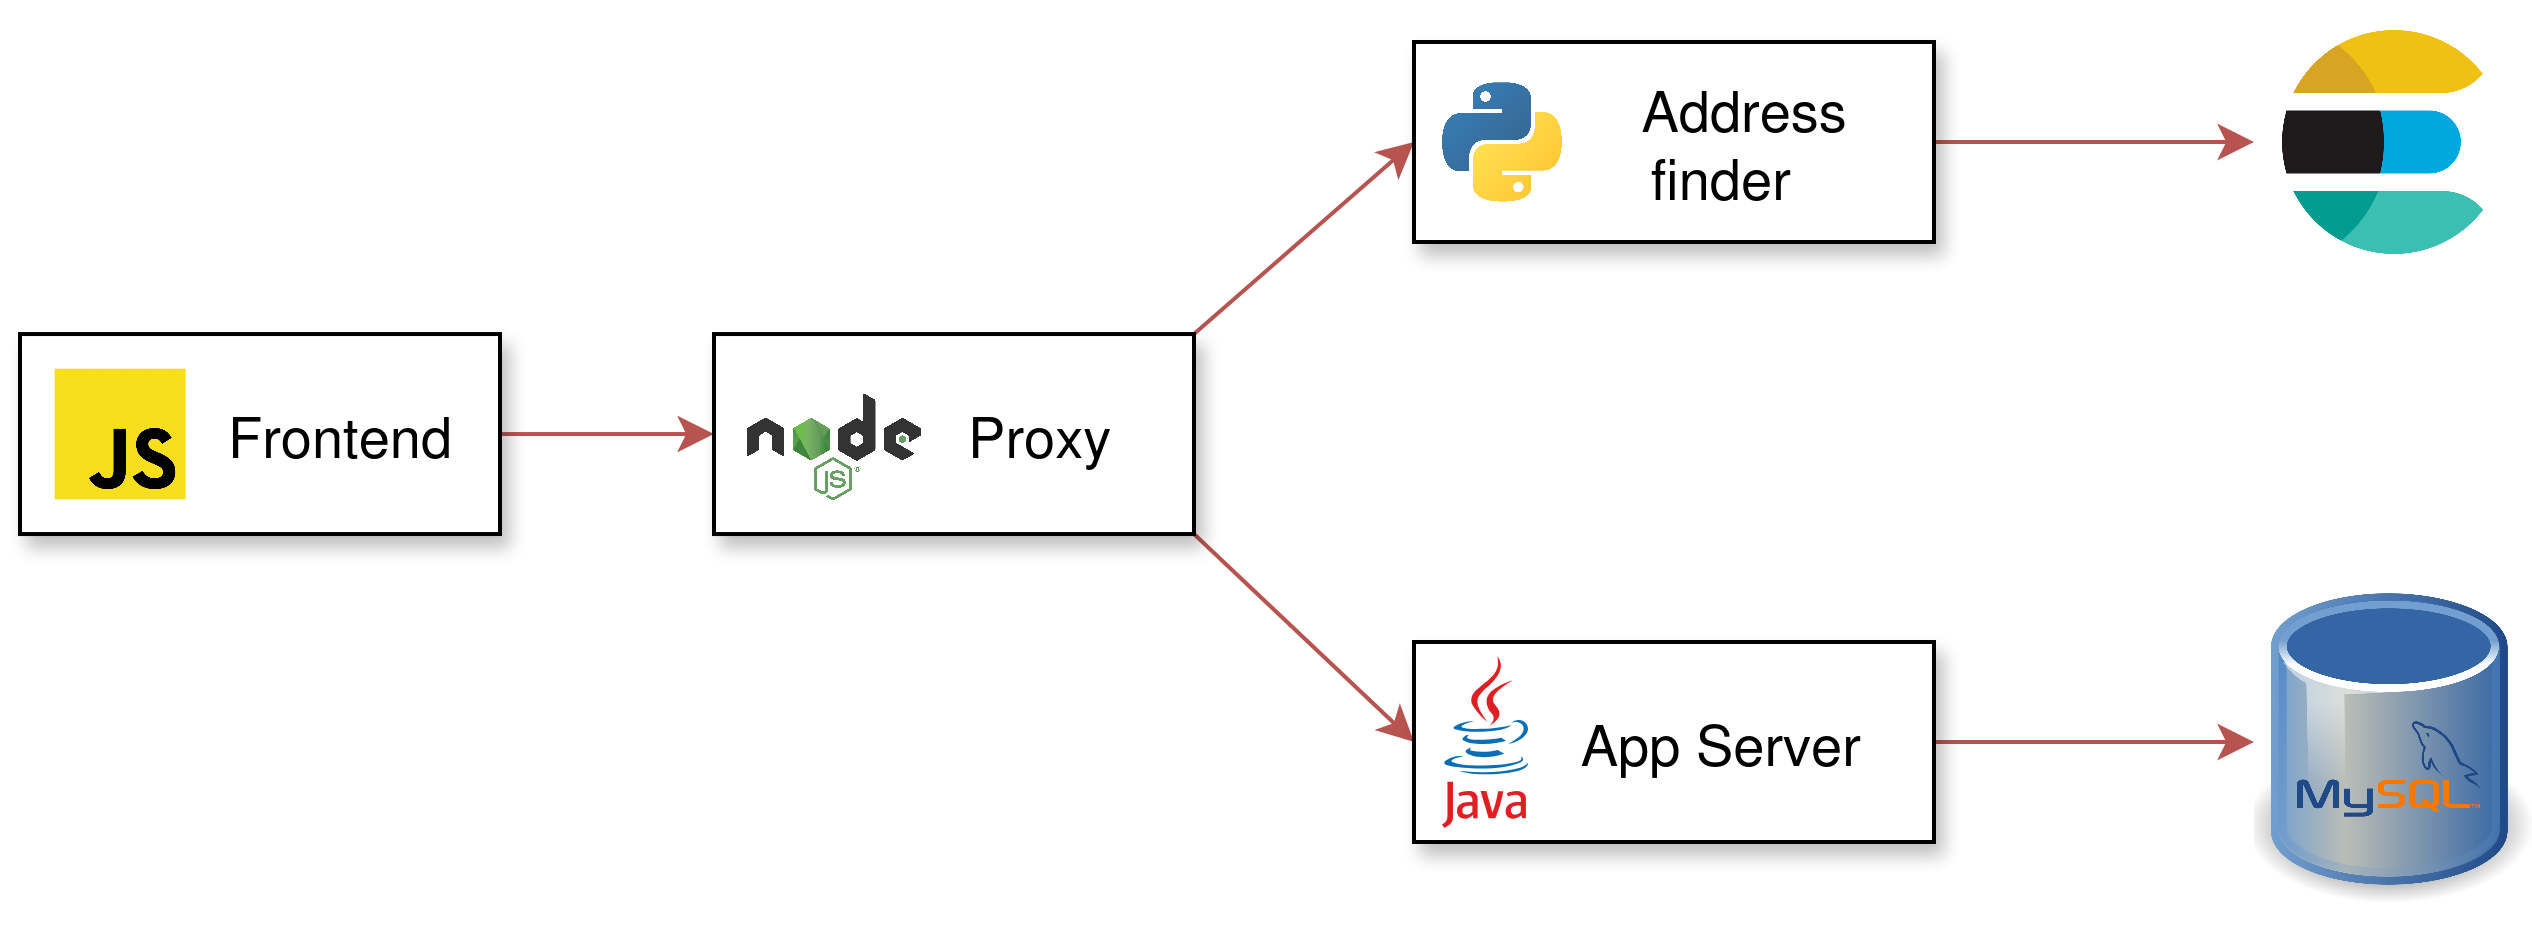
\includegraphics[width=\columnwidth]{Architettura_PetClinic.png} 
    \caption{Figura 3.1 - Architettura di Spring PetClinic}
\end{figure}


L'applicazione \emph{PetClinic} verrà quindi utilizzata come caso di studio per la validazione della soluzione di monitoraggio proposta, analizzando successivamente il modo in cui i diversi moduli architetturali interagiscono con essa.
\newpage

\subsection{User Stories e scenari di utilizzo}
Le seguenti \emph{user stories} descrivono brevemente i principali scenari di utilizzo del sistema di \gls{apm}, evidenziando gli obiettivi e le esigenze degli utenti tecnici aziendali che operano sulla piattaforma di monitoraggio.  
L'unico attore considerato è l'\emph{Observability Engineer}, figura responsabile della configurazione, analisi e manutenzione del sistema all'interno dell'infrastruttura aziendale.


\begin{center}
\captionof{table}{User stories}
\label{tab:user-stories}
\begin{tabularx}{\textwidth}{|c|X|X|}
\hline
\rowcolor[gray]{0.8}
\textbf{ID} & \textbf{User Story} & \textbf{Obiettivo} \\
\hline
\textbf{US1} & Come \emph{Observability Engineer}, voglio analizzare i tempi medi di risposta degli \emph{endpoint} dell'applicazione per individuare colli di bottiglia o degradi di \emph{performance}. & Ottimizzare le prestazioni applicative. \\
\hline
\textbf{US2} & Come \emph{Observability Engineer}, voglio monitorare l'utilizzo di \gls{cpug}, memoria e connessioni per valutare la stabilità del sistema e prevenire sovraccarichi. & Garantire la corretta gestione delle risorse. \\
\hline
\textbf{US3} & Come \emph{Observability Engineer}, voglio rilevare e classificare errori e anomalie dai \emph{log} e dalle tracce distribuite per identificare rapidamente le cause dei malfunzionamenti. & Migliorare l'affidabilità del sistema. \\
\hline
\textbf{US4} & Come \emph{Observability Engineer}, voglio configurare regole di \emph{alerting} in \emph{Kibana} per essere notificato in caso di anomalie o soglie critiche superate. & Ridurre i tempi di risposta agli incidenti. \\
\hline
\textbf{US5} & Come \emph{Observability Engineer}, voglio visualizzare le metriche aggregate in \emph{dashboard} personalizzate in modo da avere una panoramica chiara dello stato del sistema. & Facilitare l'analisi e la comunicazione dei risultati. \\
\hline

\end{tabularx}
\end{center}

\vspace{1em}


%\section{Conclusioni}
%Il presente capitolo ha illustrato l'analisi dei requisiti del sistema di \gls{apm}, la loro classificazione e la relativa mappatura sulle componenti principali dell'architettura prevista.  

    \chapter{Tecnologie e principi teorici}
\label{cap:tecnologie-principi-teorici}

\intro{Il capitolo presenta il quadro teorico e tecnologico di riferimento del progetto, descrivendo i principali approcci e strumenti per il monitoraggio delle prestazioni applicative. Vengono illustrate le tecnologie analizzate e le motivazioni che hanno guidato la scelta della soluzione, in relazione ai requisiti e agli obiettivi del sistema di osservabilità sviluppato.}\\

\section{APM e Observability}
\label{sec:apm-observability}
Definizione, Obiettivi e componenti tipici di un sistema APM.


\section{Approcci e tecnologie per il monitoraggio}
\label{sec:approcci-tecnologie-monitoraggio}

\subsection{Approcci principali}


\subsection{Tecnologie e piattaforme note}


\section{Tecnologie e strumenti}
\label{sec:tecnologie-strumenti}
Di seguito viene data una panoramica delle tecnologie e degli strumenti utilizzati.

\subsection{Elastic Stack}

\subsection*{Elasticsearch}
Elasticsearch è un motore di ricerca e analisi distribuito basato su \emph{Apache Lucene}, progettato per gestire grandi volumi di dati in tempo reale. Fornisce funzionalità avanzate di ricerca \emph{full-text}, analisi dei dati e aggregazioni, rendendolo ideale per applicazioni di monitoraggio, analisi dei \emph{log} e \emph{business intelligence}. Elasticsearch supporta un'architettura scalabile e flessibile, consentendo di distribuire i dati su più nodi e cluster per garantire alta disponibilità e prestazioni elevate.

\begin{figure}[H] 
    \centering 
    
\includegraphics[width=4cm]{/logos/elasticsearch.png} 
    \caption{Figura 4.1 - Elasticsearch}
\end{figure}


\subsection*{Kibana}
Kibana è uno strumento di visualizzazione e analisi dei dati open source, progettato per lavorare in stretta integrazione con Elasticsearch. Fornisce un'interfaccia utente intuitiva che consente agli utenti di creare \emph{dashboard} interattive, visualizzare grafici, mappe e tabelle, e analizzare i dati in tempo reale. Kibana supporta una vasta gamma di visualizzazioni personalizzabili e offre funzionalità avanzate come il filtraggio dei dati, la ricerca \emph{full-text} e l'esplorazione delle relazioni tra i dati, rendendolo uno strumento potente per l'analisi dei \emph{log}, il monitoraggio delle prestazioni e la \emph{business intelligence}.

\begin{figure}[H] 
    \centering 
    
\includegraphics[width=4cm]{/logos/kibana.png} 
    \caption{Figura 4.2 - Kibana}
\end{figure}


\subsection*{Beats}
Beats è una piattaforma leggera di raccolta dati open source sviluppata da Elastic, progettata per inviare dati da diverse fonti a Elasticsearch o Logstash. I \emph{Beats} sono agenti specializzati che raccolgono specifici tipi di dati, come \emph{log} di sistema, metriche di rete, dati di sicurezza e altro ancora. Grazie alla loro architettura modulare e alla facilità di configurazione, i \emph{Beats} consentono agli utenti di monitorare e analizzare rapidamente i dati provenienti da ambienti distribuiti e complessi.


\subsection*{Elastic Agent e Fleet}
Elastic Agent è un agente unificato sviluppato da Elastic che consente di raccogliere, monitorare e proteggere i dati da diverse fonti in modo semplice ed efficiente. Integrando funzionalità di raccolta dati, sicurezza e monitoraggio, Elastic Agent semplifica la gestione degli agenti e riduce la complessità operativa. Fleet è una funzionalità di gestione centralizzata all'interno di Kibana che consente di distribuire, configurare e monitorare gli Elastic Agent in modo scalabile e automatizzato. Attraverso Fleet, gli utenti possono gestire facilmente le policy di raccolta dati, aggiornare gli agenti e monitorare lo stato della loro infrastruttura da un'unica interfaccia.


\subsection*{OpenTelemetry}

\begin{figure}[H] 
    \centering 
    
\includegraphics[width=4cm]{/logos/OpenTelemetry.png} 
    \caption{Figura 4.3 - OpenTelemetry}
\end{figure}

\subsection*{Elastic APM e APM Server}
\begin{figure}[H] 
    \centering 
    
\includegraphics[width=4cm]{/logos/ElasticAPM.png} 
    \caption{Figura 4.4 - Elastic APM}
\end{figure}

\subsection*{RUM Agent e Synthetic Monitoring}

\subsection*{MCP}


\subsection{Linguaggi di programmazione}
\subsection*{Python}
\begin{figure}[H] 
    \centering 
    
\includegraphics[width=4cm]{/logos/Python_logonormal.png} 
    \caption{Figura 4.5 - Python}
\end{figure}


\subsection*{JavaScript}
\begin{figure}[H] 
    \centering 
    
\includegraphics[width=4cm]{/logos/javascript.png} 
    \caption{Figura 4.6 - JavaScript}
\end{figure}


\subsection*{Java}
\begin{figure}[H] 
    \centering 
    
\includegraphics[width=4cm]{/logos/java.png} 
    \caption{Figura 4.7 - Java}
\end{figure}


\subsection{Framework e librerie}
\subsection*{Node.js}
\begin{figure}[H] 
    \centering 
    
\includegraphics[width=4cm]{/logos/nodeJS.png} 
    \caption{Figura 4.8 - Node.js}
\end{figure}


\subsection*{Spring Boot}
\begin{figure}[H] 
    \centering 
    
\includegraphics[width=4cm]{/logos/spring.png} 
    \caption{Figura 4.9 - Spring}
\end{figure}


\subsection*{Selenium}
\begin{figure}[H] 
    \centering 
    
\includegraphics[width=4cm]{/logos/selenium.png} 
    \caption{Figura 4.10 - Selenium}
\end{figure}


\subsection{Strumenti di sviluppo}
\subsection*{VSCode}
\begin{figure}[H] 
    \centering 
    
\includegraphics[width=4cm]{/logos/vscode.png} 
    \caption{Figura 4.11 - VSCode}
\end{figure}


\subsection{Database}
\subsection*{MySQL}
\begin{figure}[H] 
    \centering 
    
\includegraphics[width=4cm]{/logos/Mysql_barattolo.png} 
    \caption{Figura 4.12 - MySQL}
\end{figure}


\section{Criteri di scelta della soluzione}
\label{sec:criteri-scelta-soluzione}


\section{Integrazione con l'ambiente esistente}
\label{sec:integrazione-ambiente-esistente}


%\section{Ciclo di vita del software}
%\label{sec:ciclo-vita-software}

%\section{Progettazione}
%\label{sec:progettazione}

%\subsubsection{Namespace 1} %**************************
%Descrizione namespace 1.

%\begin{namespacedesc}
    %\classdesc{Classe 1}{Descrizione classe 1}
    %\classdesc{Classe 2}{Descrizione classe 2}
%\end{namespacedesc}


%\section{Design Pattern utilizzati}

%\section{Codifica}

    \input{chapters/product-design}
    \input{chapters/conclusioni}

    \appendix
    \input{appendix/appendice-a}

    \backmatter
    \printglossary[type=\acronymtype, title=Acronimi e abbreviazioni, toctitle=Acronimi e abbreviazioni]
    \printglossary[type=main, title=Glossario, toctitle=Glossario]

    \input{appendix/bibliography}
\end{document}
